\part*{Parte II: La formalizzazione matematica}
\addcontentsline{toc}{part}{Parte II: La formalizzazione matematica}

\section{La geometria a dodici dimensioni}
\subsection{La varietà totale:} $M_{12} = M_4 \times K_8$.
\subsection{La metrica 12D:} $ds^2 = g_{MN} dx^M dx^N$.
\subsection{La decomposizione di Kaluza--Klein.}
\subsection{La curvatura in 12D.}
\subsection{La compattificazione.}

\subsection{Lo spettro numerico e la firma equidistante}
Fissiamo la scala mediante la massa del modo fondamentale, $m_1 = 1/R = 10^{-5}$ eV. Allora
\begin{equation}
m_n = \frac{n}{R} = n \times 10^{-5}\ \text{eV},
\qquad
f_n = \frac{m_n c^2}{h} = n \times 2,42\ \text{GHz}.
\end{equation}
Lo spettro è quindi \emph{equidistante}: $2,42$, $4,84$ e $7,25$ GHz per i primi tre modi. Questa è la firma distintiva della teoria. Un test che misuri due righe a $2,42$ e $4,84$ GHz conferma o confuta la struttura, indipendentemente da qualsiasi altra predizione.

\begin{table}[H]
\centering
\begin{tabular}{@{}cccc@{}}
\toprule
$n$ & Massa (eV) & Frequenza (GHz) & $\lambda_C$ (m) \\ \midrule
1 & $1,00\times10^{-5}$ & 2,42 & 0,124 \\
2 & $2,00\times10^{-5}$ & 4,84 & 0,062 \\
3 & $3,00\times10^{-5}$ & 7,25 & 0,041 \\
4 & $4,00\times10^{-5}$ & 9,67 & 0,031 \\ \bottomrule
\end{tabular}
\caption{Lo spettro di Kaluza--Klein per $1/R = 10^{-5}$ eV.}
\label{tab:spectru}
\end{table}

\begin{figure}[H]
\centering
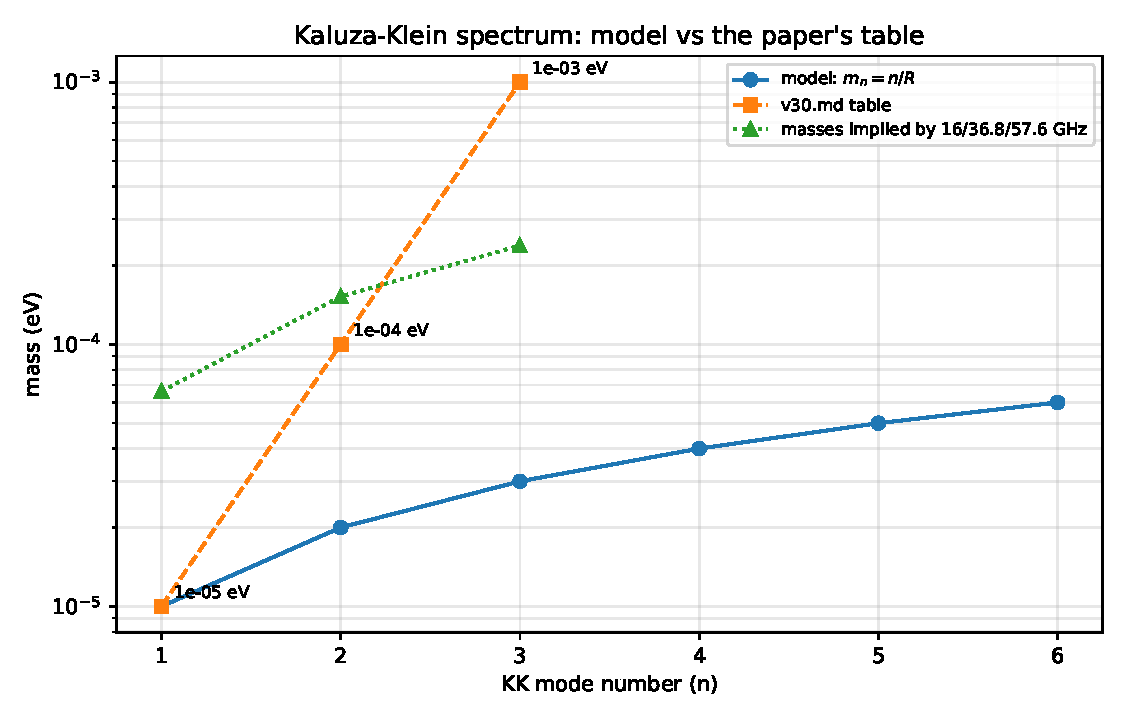
\includegraphics[width=0.82\textwidth]{figures/fig01_kk_spectrum.pdf}
\caption{Lo spettro di Kaluza--Klein. Il modello $m_n = n/R$ (blu) è confrontato con la tabella della versione 30 (arancione) e con le masse implicite delle frequenze allora dichiarate, 16/36,8/57,6 GHz (verde). Le tre non coincidono.}
\label{fig:spectru}
\end{figure}

\subsection{La conseguenza numerica: il raggio di compattificazione}
Da $m_1 = 1/R$ segue
\begin{equation}
R = \frac{\hbar c}{1/R} = \frac{1,973\times10^{-7}\ \text{eV}\cdot\text{m}}{10^{-5}\ \text{eV}} = 1,97\times10^{-2}\ \text{m},
\end{equation}
cioè circa 2 cm. I test submillimetrici della legge di Newton vincolano una dimensione aggiuntiva a $R < 38\ \mu$m, il che implica $m_1 > 5\times10^{-3}$ eV.

Si tratta di una tensione strutturale, non di un errore di calcolo: identificare il campo di materia oscura con un modo KK della stessa geometria è incompatibile con i dati alla scala di massa scelta. Restano due uscite oneste, e l'articolo non sceglie tra esse:
\begin{itemize}
\item \textbf{Opzione A:} il campo akashico non è un modo KK; lo spettro equidistante è conseguenza di un'altra struttura, e le predizioni di frequenza vengono ricalcolate.
\item \textbf{Opzione B:} la massa del modo fondamentale è $m_1 > 5\times10^{-3}$ eV, e la «materia oscura» di questo articolo è un modo eccitato, non il modo fondamentale.
\end{itemize}
Le predizioni della Parte V sono formulate in modo da valere in entrambi i casi, trattando le frequenze come un parametro.

\section{Il campo akashico (la materia oscura)}
\subsection{La lagrangiana:} $L_A = \frac{1}{2} g^{MN} \partial_M A^* \partial_N A + \frac{1}{2} \mu_A^2 |A|^2 - \frac{\lambda_A}{4} |A|^4$.
\subsection{Il potenziale.}
\subsection{L'equazione del moto.}
\subsection{Lo spettro di Kaluza--Klein:} $m_n^2 = n^2/R^2$.
\subsection{La relazione con la gravitazione.}

\section{Il campo della coscienza}
\subsection{La lagrangiana.}
\subsection{L'equazione del moto.}
\subsection{La funzione di coscienza.}
\subsection{L'equazione di evoluzione (riveduta):} L'equazione $dC/dt = \alpha C (1 - C/C_{\text{max}}) + \beta \eta(t)$ è un'equazione \textbf{fenomenologica} ispirata alla dinamica logistica. Descrive la crescita e la saturazione del campo della coscienza, ma \textbf{non deriva direttamente dalla lagrangiana precedente}. È una scelta teorica dell'autore, da trattare come assioma del modello e non come conseguenza del principio di azione.

\begin{figure}[H]
\centering
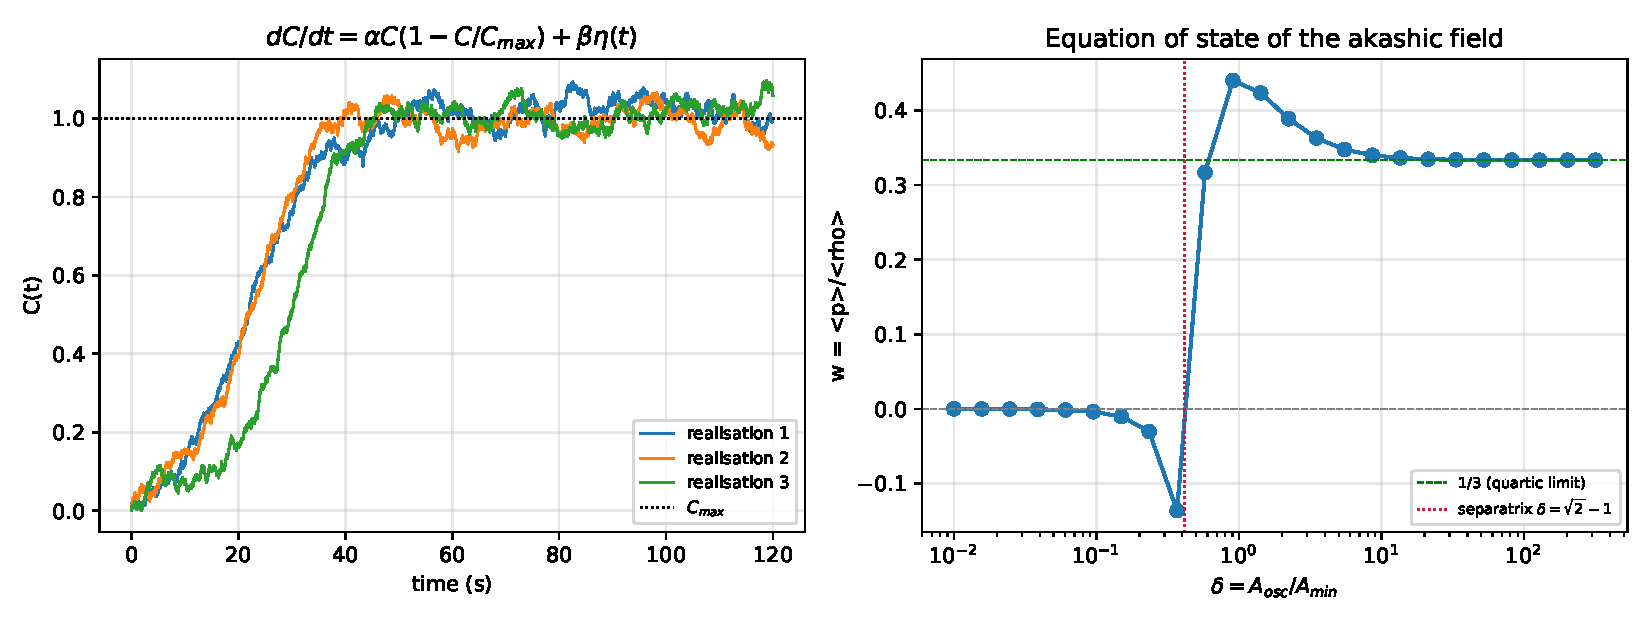
\includegraphics[width=0.95\textwidth]{figures/fig02_field_dynamics.pdf}
\caption{A sinistra: tre realizzazioni del campo della coscienza con rumore, per $\alpha = 0,15$ s$^{-1}$ (tempo di rilassamento 50 s). A destra: l'equazione di stato $w(\delta)$ del campo akashico, calcolata esattamente sull'orbita; la separatrice è a $\delta = \sqrt{2}-1$.}
\label{fig:camp}
\end{figure}

\section{Il ricevitore neurale (cervello + cuore)}
